\documentclass[iop]{emulateapj-rtx4}


%\documentclass[12pt]{article}
%\pdfpagewidth 8.5in
%\pdfpageheight 11in 
%\setlength\topmargin{0in}
%\setlength\headheight{0in}
%\setlength\headsep{0in}
%\setlength\textheight{9in}
%\setlength\textwidth{6.5in}
%\setlength\oddsidemargin{0in}
%\setlength\evensidemargin{0in}

\usepackage{graphicx}
\usepackage{amssymb}

%\usepackage{multicol}
%\usepackage{sidecap}
%\usepackage{ragged2e}

%\usepackage{caption}
%\usepackage{subcaption}

\usepackage{wrapfig}
\usepackage{setspace}
\usepackage{subfigure}
\usepackage{mathtools}


%\newcommand{\rms}[1]{\langle #1 \rangle}
%\renewcommand{\baselinestretch}{1.5}
%\renewcommand{\thefootnote}{\roman{footnote}}

\graphicspath{{paper_figures//}}


\frenchspacing

\begin{document}

%\onehalfspacing

\title{Probing the CGM in the nearby Universe in Ly$\alpha$ absorption: Discovery of an gas absorption-velocity dichotomy}
\author{David M. French, Bart P. Wakker}
\affil{Department of Astronomy, University of Wisconsin - Madison}

%\affil{Department of Astronomy, University of Wisconsin - Madison; frenchd@astro.wisc.edu}


\begin{abstract}

We present initial results from an ongoing large-scale study of the circumgalactic medium in the nearby Universe ($cz < 10,000 km/s$), using archive Cosmic Origins Spectrograph (COS) sightlines of background QSOs. This initial sample contains 35 sight lines, yielding 154 Ly$\alpha$ systems, 46 of which we have paired with nearby galaxies. We introduce a likelihood parameter to quantitatively predict the galaxy responsible for measured absorption in a reproducible way. We find a dichotomy in the equivalent widths (EW) of absorption systems around $\Delta v = v_{galaxy} - v_{gas}$, with positive $\Delta v$ absorption EW = $366 \pm 15$m\AA, and negative $\Delta v$  absorption EW = $192 \pm 12$m\AA. We also find a preference for absorption around highly inclined galaxies, but little evidence of azimuthal dependence.


%Galaxies must accrete gas from the intergalactic medium (IGM) in order to sustain star formation at observed levels. In order to understand this complex process, and how it influences galaxy evolution, it is necessary to understand the physical conditions and distribution of the gas around galaxies, known as the circumgalactic medium (CGM). For my thesis, I propose to use archival spectra of bright background QSOs taken by the Cosmic Origins Spectrograph (COS) on the Hubble Space Telescope (HST) to directly probe the CGM of galaxies in the nearby Universe. I will supplement this spectral data with observations of these galaxies taken by the WIYN and SALT telescopes. This proposed program will be the largest and most statistically significant survey of the local CGM to date.

\end{abstract}
\keywords{IGM, CGM, galaxies}


%\section{THINGS I STILL NEED}
%
%- target list table
%- galaxy table completeness plot
%- breakdown of systems into single galaxy (certain), multiple galaxies (probable), multiple galaxies (ambiguous)
%- mean azimuth, blue and red azimuths
%- mean inclination, blue and red inclinations
%- mean Lstar for associated galaxies of each type


\section{Introduction}


It is well known that galaxies must continue to accrete gas throughout their lifetimes in order to sustain observed levels of star formation (e.g. Erb 2008, Putman et al. 2009b). This additional gas must come from the diffuse intergalactic medium (IGM), where the majority of the baryons in the universe reside (CITATION?). How exactly this IGM gas eventually falls into the halos and disks of galaxies is still highly uncertain, as observational constraints are hard to come by. Because of the diffuse nature of IGM gas, it is most readily and sensitively detected as absorption in the spectra of background active galactic nuclei (AGN). The advent of the sensitive UV spectrographs STIS and COS on the Hubble Space Telescope (HST) have provided a wealth of information on the properties and distribution of both the ions of heavy elements as well as the Lyman series of neutral H\,{\sc i} gas around galaxies. 

Individual concentrations of gas along a given sightline imprint a `forest' of absorption lines on the spectrum in the direction of the QSO. The metal lines trace the star formation history within the intervening gas, and neutral hydrogen lines (Ly$\alpha$) indicate both the location and velocities of outflowing gas as well as the presence of fuel for future star formation. Numerous studies using these observations have shown that Ly$\alpha$ absorbers trace individual galaxy halos (e.g. Wakker $\&$ Savage 2009, Danforth et al. 2014, Stocke et al. 2013 $\&$ 2014, Liang et al 2014, Lanzetta et al 1995, Chen et al. 1998, 2001a, Tripp et al. 1998, Steidel et al. 2010, Prochaska et al. 2011, Thom et al 2012, Tumlinson et al. 2011 $\&$ 2013). 


%It is well known now that galaxies must continue to accrete gas throughout their lifetimes in order to sustain observed levels of star formation (e.g., see Erb 2008, Putman et al. 2009b). This additional gas comes from the diffuse intergalactic medium (IGM), where the majority of the baryons in the universe reside. In order to understand the life cycle of this gas and its effect on the evolution of nearby galaxies, it is necessary to understand its physical properties such as densities, temperatures, motions, and its interactions with the galaxies. This can be accomplished by analyzing lines of sight toward background QSOs.

%The current standard model of structure formation is given by $\Lambda$CDM cosmology, which predicts the hierarchical growth of large scale structures seeded by initial fluctuations in the dark matter background. In this picture, both galaxies and neutral H\,{\sc i} follow the same underlying density profile. Wakker et al. (2015, submitted) have provided some observational evidence for this, showing that Ly$\alpha$ absorption strength traces the large-scale distribution of galaxies in a Cosmic Web filament. In addition, numerous previous studies have shown that Ly$\alpha$ absorbers also trace individual galaxy halos (e.g. Wakker $\&$ Savage 2009, Danforth et al. 2014, Stocke et al. 2013, Liang et al 2014, Lanzetta et al 1995, Chen et al. 1998, 2001a, Tripp et al. 1998, Steidel et al. 2010, Prochaska et al. 2011, Thom et al 2012). 


Some recent studies find that about half of Ly$\alpha$ absorbers lie within galaxy haloes, at impact parameters $\rho<350$ kpc (C\^{o}t\'{e} et al. 2005, Prochaska et al. 2006). In addition, Wakker $\&$ Savage (2009) find that for 90$\%$ of L$>0.1L_{\**}$ galaxies an absorber lies within 400 kpc and 400 km/s, and all galaxies have a Ly$\alpha$ absorber within 1.5 Mpc. Higher redshift studies, such as Rudie et al. (2012) at $2<z<3$, find evidence for an elevated density of absorbers up to 2 Mpc from galaxies. Wakker $\&$ Savage (2009) also confirmed a previously suggested correlation between Ly$\alpha$ absorption linewidth ($W$) and impact parameter $\rho$, observing that the broadest lines (FWHM $>$150 km/s) are only seen within 350 kpc of a galaxy, while at $\rho>1$ Mpc, only lines with FWHM $<75$ km/s occur.


In addition, studying the enrichment of galaxy halos is necessary for constraining outflow models and informing stellar feedback prescriptions. Directly measuring the velocity field and column densities of absorbers as a function of impact parameter and orientation around galaxies would provide the clearest evidence of inflow or outflow activity, but results are still uncertain. Kacprzak et al. (2011) claim to find that Mg\,{\sc ii} equivalent widths correlate with galaxy inclination, but Mathes et al. (2014) find no such correlation for Ly$\alpha$ and O\,{\sc vi} absorbers. Furthermore, we should expect outflowing gas to be more highly enriched and trace the metallicity of the associated galaxy, with inflowing gas instead appearing only in H\,{\sc i}. Both Stocke et al. (2013) and Liang $\&$ Chen (2014) find an ``edge'' to heavy ion absorption at $\sim0.5R_h$, but with Ly$\alpha$ covering fractions of $\sim0.75-1$ continuing out to $R_{vid}$. However, Mathes et al. (2014) measures O\,{\sc vi} absorption out to $\sim3$ $D_{gal}/R_{vir}$. 


Recent results from Kacprzak et al. (2011 $\&$ 2012) suggest that absorbing systems have a preferred orientation with respect to the major and minor axes of the galaxies they are associated with. This could be evidence of inflows and outflows, or an effect of the global structure of galaxy halos, but the statistics are not yet good enough to provide consistent answers. A larger-scale study of inclination and azimuthal angles vs. absorber properties for the largest galaxies in the nearby universe, where it is possible to obtain inclinations and unambiguous absorber associations, is needed in order to elucidate the distribution of absorbing systems around galaxies.


These previous studies have suffered from small sample sizes (e.g. Mathes et al. 2014 use 14 galaxies, Stocke et al. 2013 use 11, Werk et al. 2014 use 44), and incompleteness due to their higher mean redshifts (e.g. the Mathes et al. 2014 sample is $0.12 <z<0.67$, and Werk et al. 2014 are complete to $\sim L^{\**}$ at $z\sim0.2$). To address these shortcomings, we are conducting a large survey of the properties of intergalactic gas in the nearby universe, where we have good and relatively complete information on both faint and bright galaxies, in order to reveal how the IGM and galaxies affect each other. We are taking advantage of the over 300 archived QSO and Seyfert spectra taken by the Cosmic Origins Spectrograph (COS) on the Hubble Space Telescope (HST), combined with the wealth of information available for the $\sim100,000$ galaxies with $cz<10,000$ km/s found in the NASA Extragalactic Database (NED) to probe the environment of absorbing gas systems in the nearby universe. This approach allows for an unbiased understanding of the distribution of the gas around galaxies, which requires looking for both detections and non-detections of gas, both near as well as far away from galaxies.

This paper presents initial results from our pilot study of 35 COS sight lines, chosen for their proximity to large galaxies and ease of spectral feature identification. This paper is organized as follows: in Section 2 we present the data and analysis techniques, in Section 3 we present the results, and in Section 4 we discuss possible interpretations of our results.

%The relationship between the galaxies and the IGM is usually studied by looking for galaxies that lie near the redshift of detected absorption lines. This approach has value, but is incomplete; it does not allow for an unbiased understanding of the distribution of the gas around galaxies, which requires looking for both detections and non-detections of gas, both near as well as far away from galaxies.

%There are many other ongoing studies of the IGM/CGM using QSO absorption to probe galaxy halos, but this is the only study that concentrates on \textit{Ly$\alpha$ absorption in the nearby} Universe, where the galaxy sample is nearly complete, and where large angular impact parameters between absorbers and galaxies can be physically meaningful, while also being of sufficiently large scale to produce robust statistics. 


\section{Data and Analysis}

This initial pilot study contains 35 sightlines to bright QSOs observed with the Cosmic Origins Spectrograph (COS). We chose sight lines based on high S/N (generally $>$10), ease of spectral identification, and proximity to large, nearby galaxies. Several are included simply because they already have published identifications. There were no strict cutoffs for galaxy size or brightness, we simply selected the top 35 sight lines after rejecting those with lower S/N and/or more complicated features. Table \ref{target_table} summarizes the properties of the QSO targets we selected. \textbf{Should this just be a single table with all absorption features, associated galaxies and QSO info combined?}

All COS spectra for the target sight lines was obtained through the Barbara A. Mikulski Archive for Space Telescopes (MAST), and processed with the latest available version of the CALCOS pipeline \textbf{WHICH IS??}. We combined individual exposures by the method of Wakker et al. (2015, submitted), which corrects the COS wavelength scale by cross-correlating all ISM and IGM lines in each exposure. This method addresses the up to $\pm40$ km/s misalignments produced by CALCOS, and produces a corrected error array based on Poisson noise, which better matches the measured errors. We then combine multiple exposure by aligning Galactic absorption lines with 21-cm spectra, and adding up the total counts in each pixel before converting to flux using the original, average flux-count ratio at each wavelength. Spectral features were both identified by eye and by a custom identification algorithm \textbf{MORE ABOUT THIS}. Only features identified with high probability by both methods are included in this dataset.

\begin{table}[ht]\footnotesize
\begin{center}
\begin{tabular}{| l | c | c |}
 \hline
  AGN name & \textit{z} & S/N  \\
	\hline
  
 MRK290 					 	 &  0.0296	 	 &  32  \\
 SBS1537+577  				 &  0.0734	 	 &  12  \\
 3C66A 						 &  0.444		 &  24  \\
 MRC2251-178 				 &  0.0661	 	 &  29  \\
 SBS1503+570 				 &  0.3589	 	 &  11  \\
 SDSSJ080838.80+051440.0 	 	 &  0.361		 &  8  \\
 2dFGRS\_S393Z082 			 &  ERR 		 &  ERR  \\ 
 PG1211+143					 &  0.0804	 	 &  19  \\
 TON488 					 	 &  0.2564 	 &  7  \\
 SDSSJ135341.03+361948.0 	 	 &  0.147 		 &  11  \\
 MRK1014 					 &  0.163 		 &  14  \\
 RX\_J1503.2+6810 			 	 &  0.114 		 &  8  \\
 PG1302-102 					 &  0.2784 	 &  6  \\
 SBS1108+560 				 &  0.765 		 &  17  \\
 PG1216+069					 &  0.3313 	 &  24  \\
 IRAS\_Z06229-6434 			 &  0.1289 	 &  18  \\
 SDSSJ080908.13+461925.6 	 	 &  0.6563 	 &  9  \\
 TON1009 					 &  0.809 		 &  10  \\
 RX\_J1330.8+3119 			 	 &  0.241 		 &  11  \\
 SDSSJ140428.30+335342.0 	 	 &  0.549 		 &  8  \\
 RX\_J0714.5+7408 			 	 &  0.371 		 &  17  \\
 PG1121+423 					 &  0.234 		 &  24  \\
 RBS2070 					 &  0.165 		 &  25  \\
 3C351.0 						 &  0.3719 	 &  ERR  \\
 HE1228+0131 				 &  0.117 		 &  69  \\
 3C273.0 					 	 &  0.1583 	 &  97  \\
 PG1626+554 				 	 &  0.133 		 &  20  \\
 PG1307+085 				 	 &  0.155 		 &  23  \\
 PKS2005-489 				 	 &  0.071 		 &  32  \\
 CSO395 					 	 &  0.169 		 &  10  \\
 HS0624+6907 				 &  0.37 		 &  8  \\
 HE0238-1904 				 	 &  0.631 		 &  36  \\
 RBS1795 					 &  0.344 		 &  35  \\
 H1101-232 					 &  0.186 		 &  16  \\
 1H0717+714 				 	 &  0.5003 	 &  40  \\
 PG0003+158 				 	 &  0.4509 	 &  29  \\
 SBS1122+594 				 &  0.858 		 &  10  \\
\hline

\end{tabular}
\end{center}
  \vspace{-10pt}
  \caption{\small{Names, redshifts, and S/N of AGN targets.}}
  \label{target_table}
\end{table}

\subsection{Galaxy Data}
Each final, combined, and identified sightline is correlated with the galaxy environment in order to match absorption features with galaxies near the sightline. To facilitate this, we have constructed a dataset of all $z\leq 0.033$ ($v\leq 10,000$km/s) galaxies with published data available through the NASA Extragalactic Database (NED\footnote{This research has made use of the NASA/IPAC Extragalactic Database (NED) which is operated by the Jet Propulsion Laboratory, California Institute of Technology, under contract with the National Aeronautics and Space Administration.}). This dataset contains over 108,000 entries, and includes data from SDSS, 2MASS, 2dF, 6dF, RC3, and many other, smaller surveys. Our criteria for including a galaxy in this dataset is only an accurate, spectroscopic redshift which places the galaxy in the $400 \leq v \leq 10,000$km/s velocity range. This restriction naturally leads to a completeness limit of $B \lesssim 18.7$ mag \textbf{CHECK THIS}, or $\sim0.1 L_*$ on average across the sky (see Figure \ref{completeness}). For any particular region of the sky, this limit will vary some depending upon which of the larger surveys cover the region. 

\begin{figure}[ht!]
        \centering
        \vspace{-10pt}
        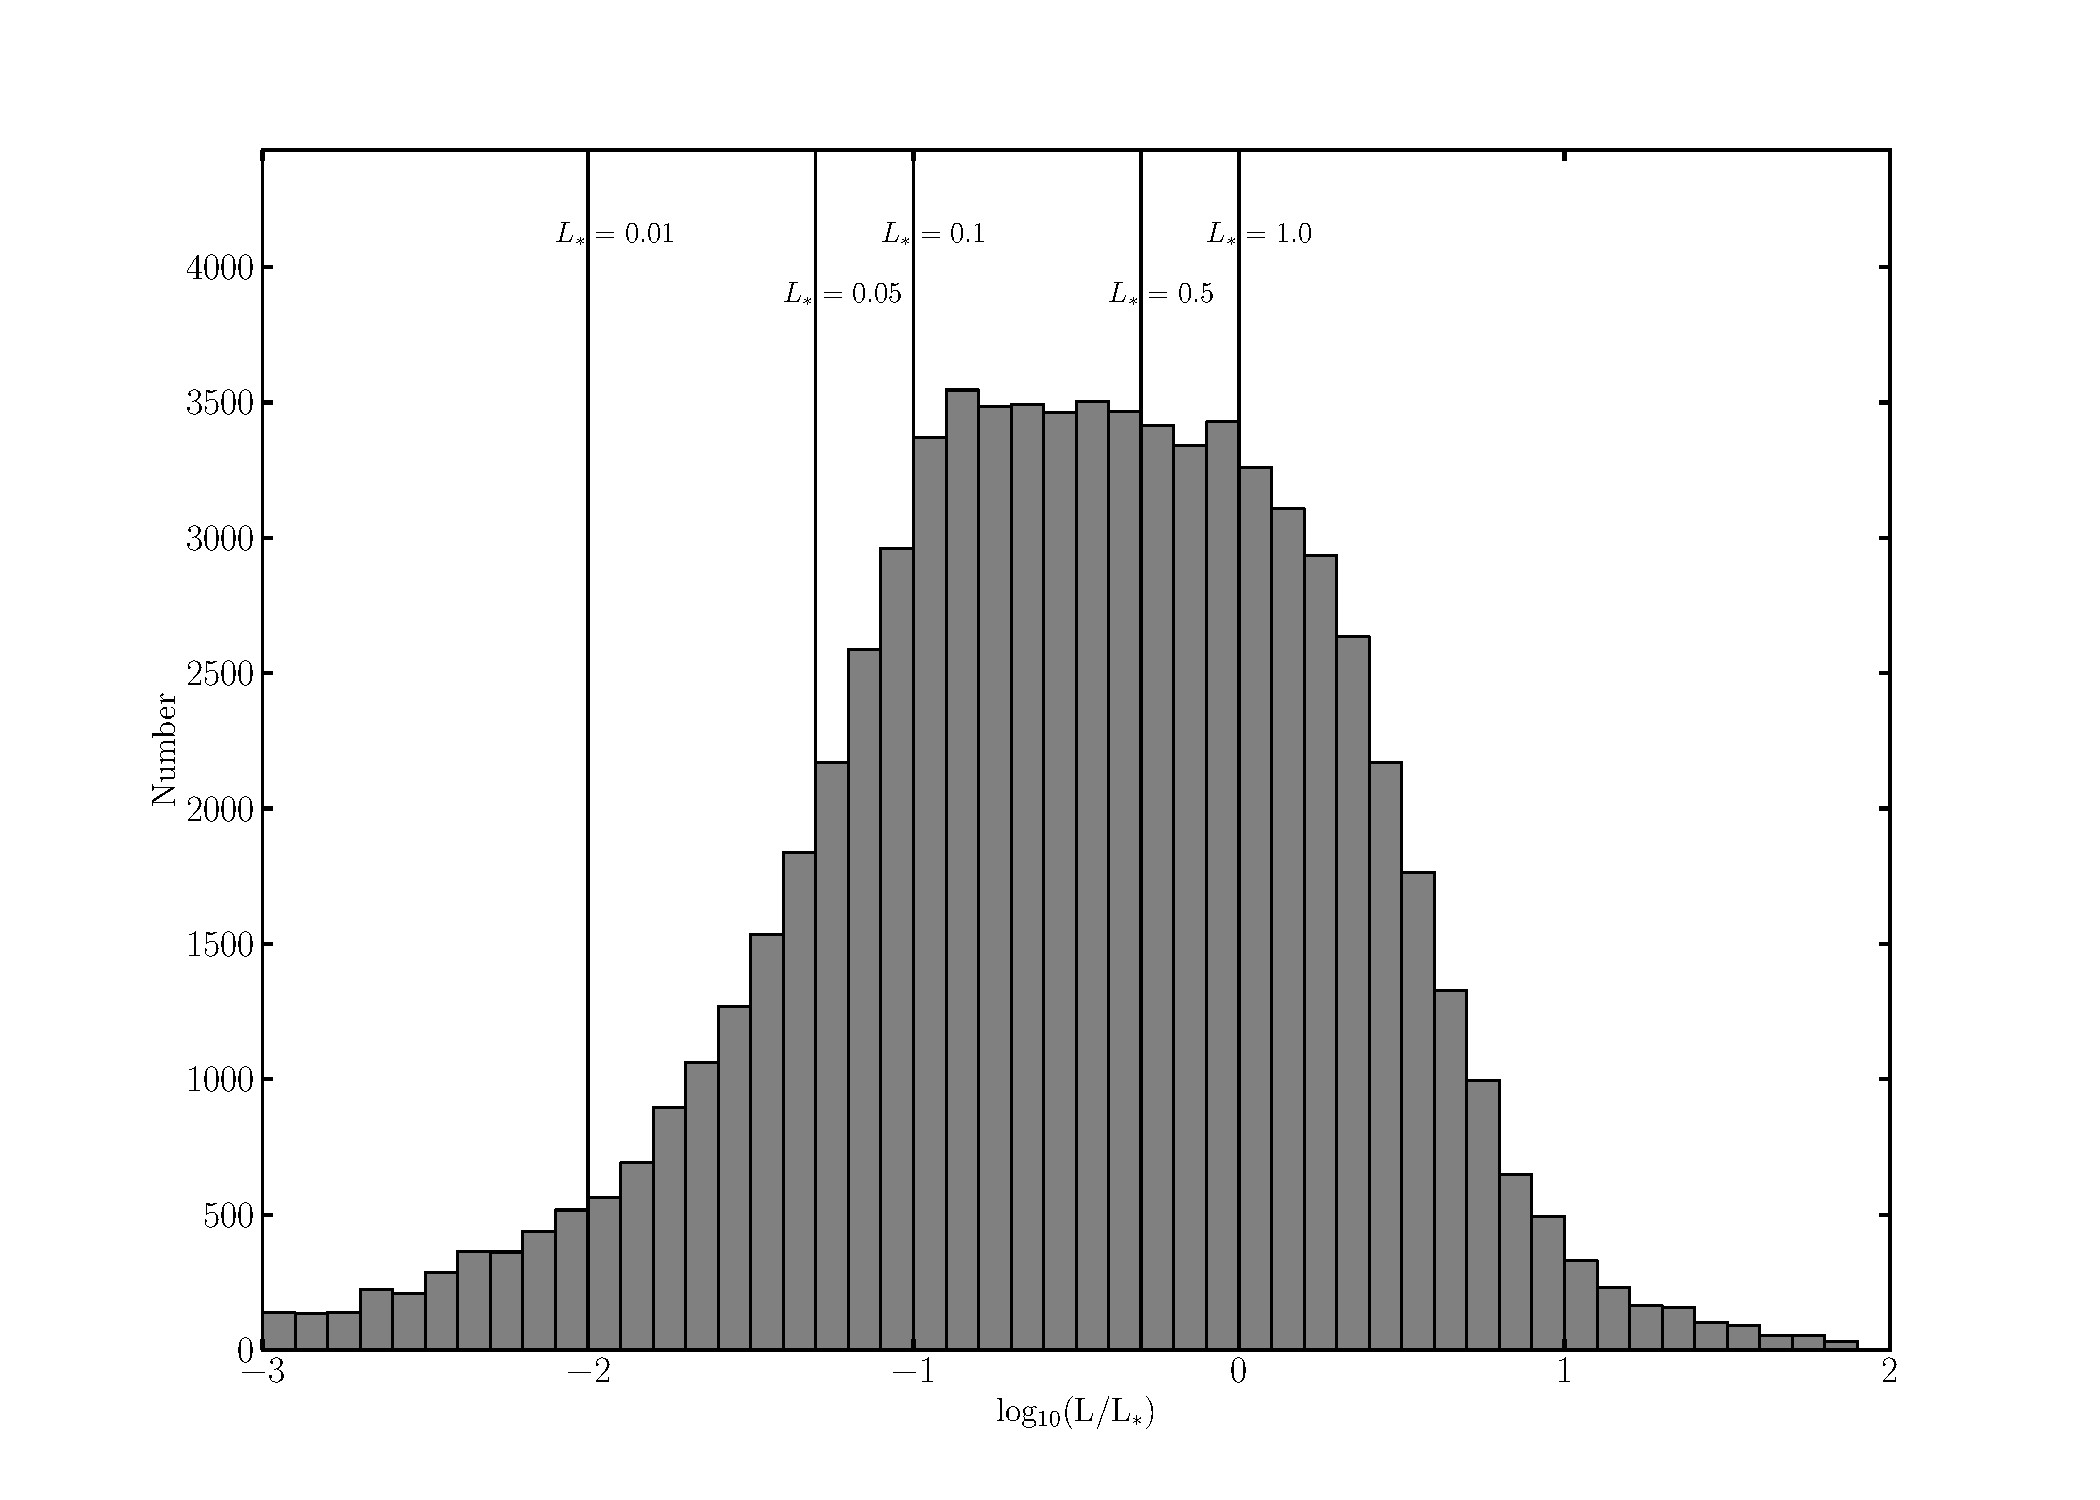
\includegraphics[width=0.52\textwidth]{completeness_hist.pdf}
        \caption{\small{Distribution of $L/L_{\**}$ values for all galaxies in the dataset. Black vertical lines highlight 1, 0.5, 0.1, 0.05 and 0.01 $L_{\**}$. The turnoff around 0.1$L_{\**}$ shows that on average, the dataset is complete to 0.1$L_{\**}$.}}
%        \vspace{-5pt}
        \label{completeness}
\end{figure} 

In addition, we have homogenized the galaxy data beyond the steps taken by NED by normalizing all measurements of galaxy inclination, position angle, and diameter to 2MASS $K$-band values. 2MASS values were chosen for this because it was an all-sky survey, and represents the largest fraction of available galaxy data. Physical galaxy diameters are derived from 2MASS $K_s$ ``total" angular diameter measurements and galaxy distances. 2MASS $K_s$ ``total" diameter estimates are surface brightness extrapolation measurements and are derived as 

\begin{equation}
r_{tot} = r' + a(ln(148)^b,
\end{equation}

\noindent where $r_{tot}$ is defined as the point where the surface brightness extends to 5 disk scale lengths, $r'$ is the starting point radius ($>5" - 10"$ beyond the nucleus, or core influence), and $a$ and $b$ are Sersic exponential function scale length parameters ($f = f_0 \exp{(-r/a)}^{(1/b)}$, see Jarret et al. 2003 for a full description). \textbf{NEEDS TO BE CHECK FOR FULL SKY} Approximately $50\%$ of all the galaxies have this 2MASS $K_s$ ``total" diameter. Of the remainder, $20\%$ have SDSS diameters, $27\%$ have no published diameter, and $3\%$ have diameters from other surveys. We convert these other estimates to 2MASS $K_s$ ``total" diameters via a simple least squares linear fit. 

We used $B$-band magnitudes to estimate each galaxy's luminosity as a ratio of $L_{\**}$ as follows:

\begin{equation}
	\frac{L}{L_{\**}} = 10^{-0.4 (M_{B} - M_{B_{\**}})}. 
\end{equation}

We adopt the CfA galaxy luminosity function by Marzke et al. (1994), which sets $B_{\**} $ = -19.57. Direct $B$ band measurements are available for $\sim 30\%$ of galaxies, and most of the rest have SDSS $g$ and $r$ magnitudes, which can be converted to $B$ via $B = g + 0.39 (g-r) + 0.21$ (Jester et al. 2005). Finally, we also compute an estimate of the virial radius of each galaxy as $log R_{vir} = 0.69 log D + 1.24$. This follows the parametrization of Stocke et al. (2013) relating a galaxy's luminosity to its virial radius, and the Wakker $\&$ Savage (2009) empirical relation between diameter and luminosity (see Wakker et al. 2015 and references therein for further details).

This homogeneous galaxy data table allows us to draw direct comparisons between the properties of the absorbers and the properties, separations, and environments of nearby galaxies, with unprecedented completeness.

\begin{figure}[h!]
\centering
  \subfigure[]{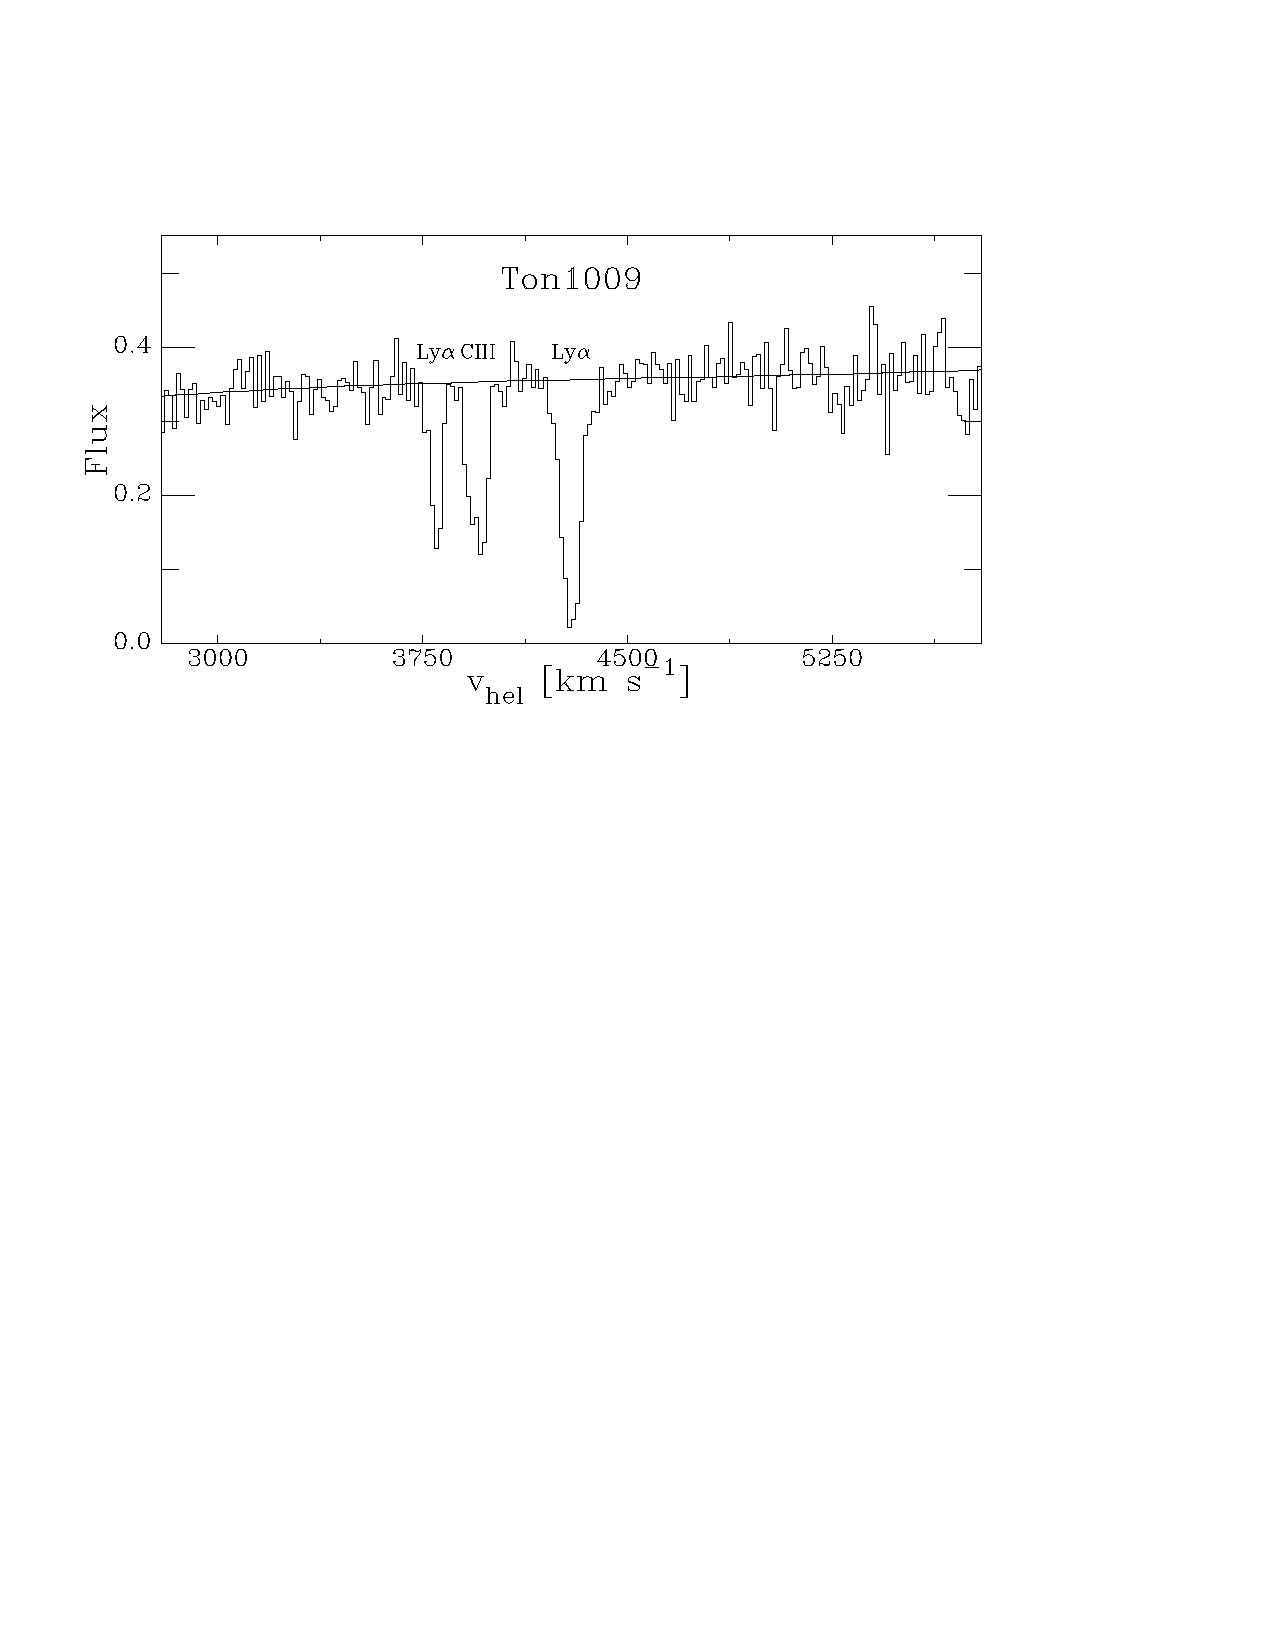
\includegraphics[width=1.\linewidth]{figTON1009_crop.pdf}}{\label{line}}
  \subfigure[]{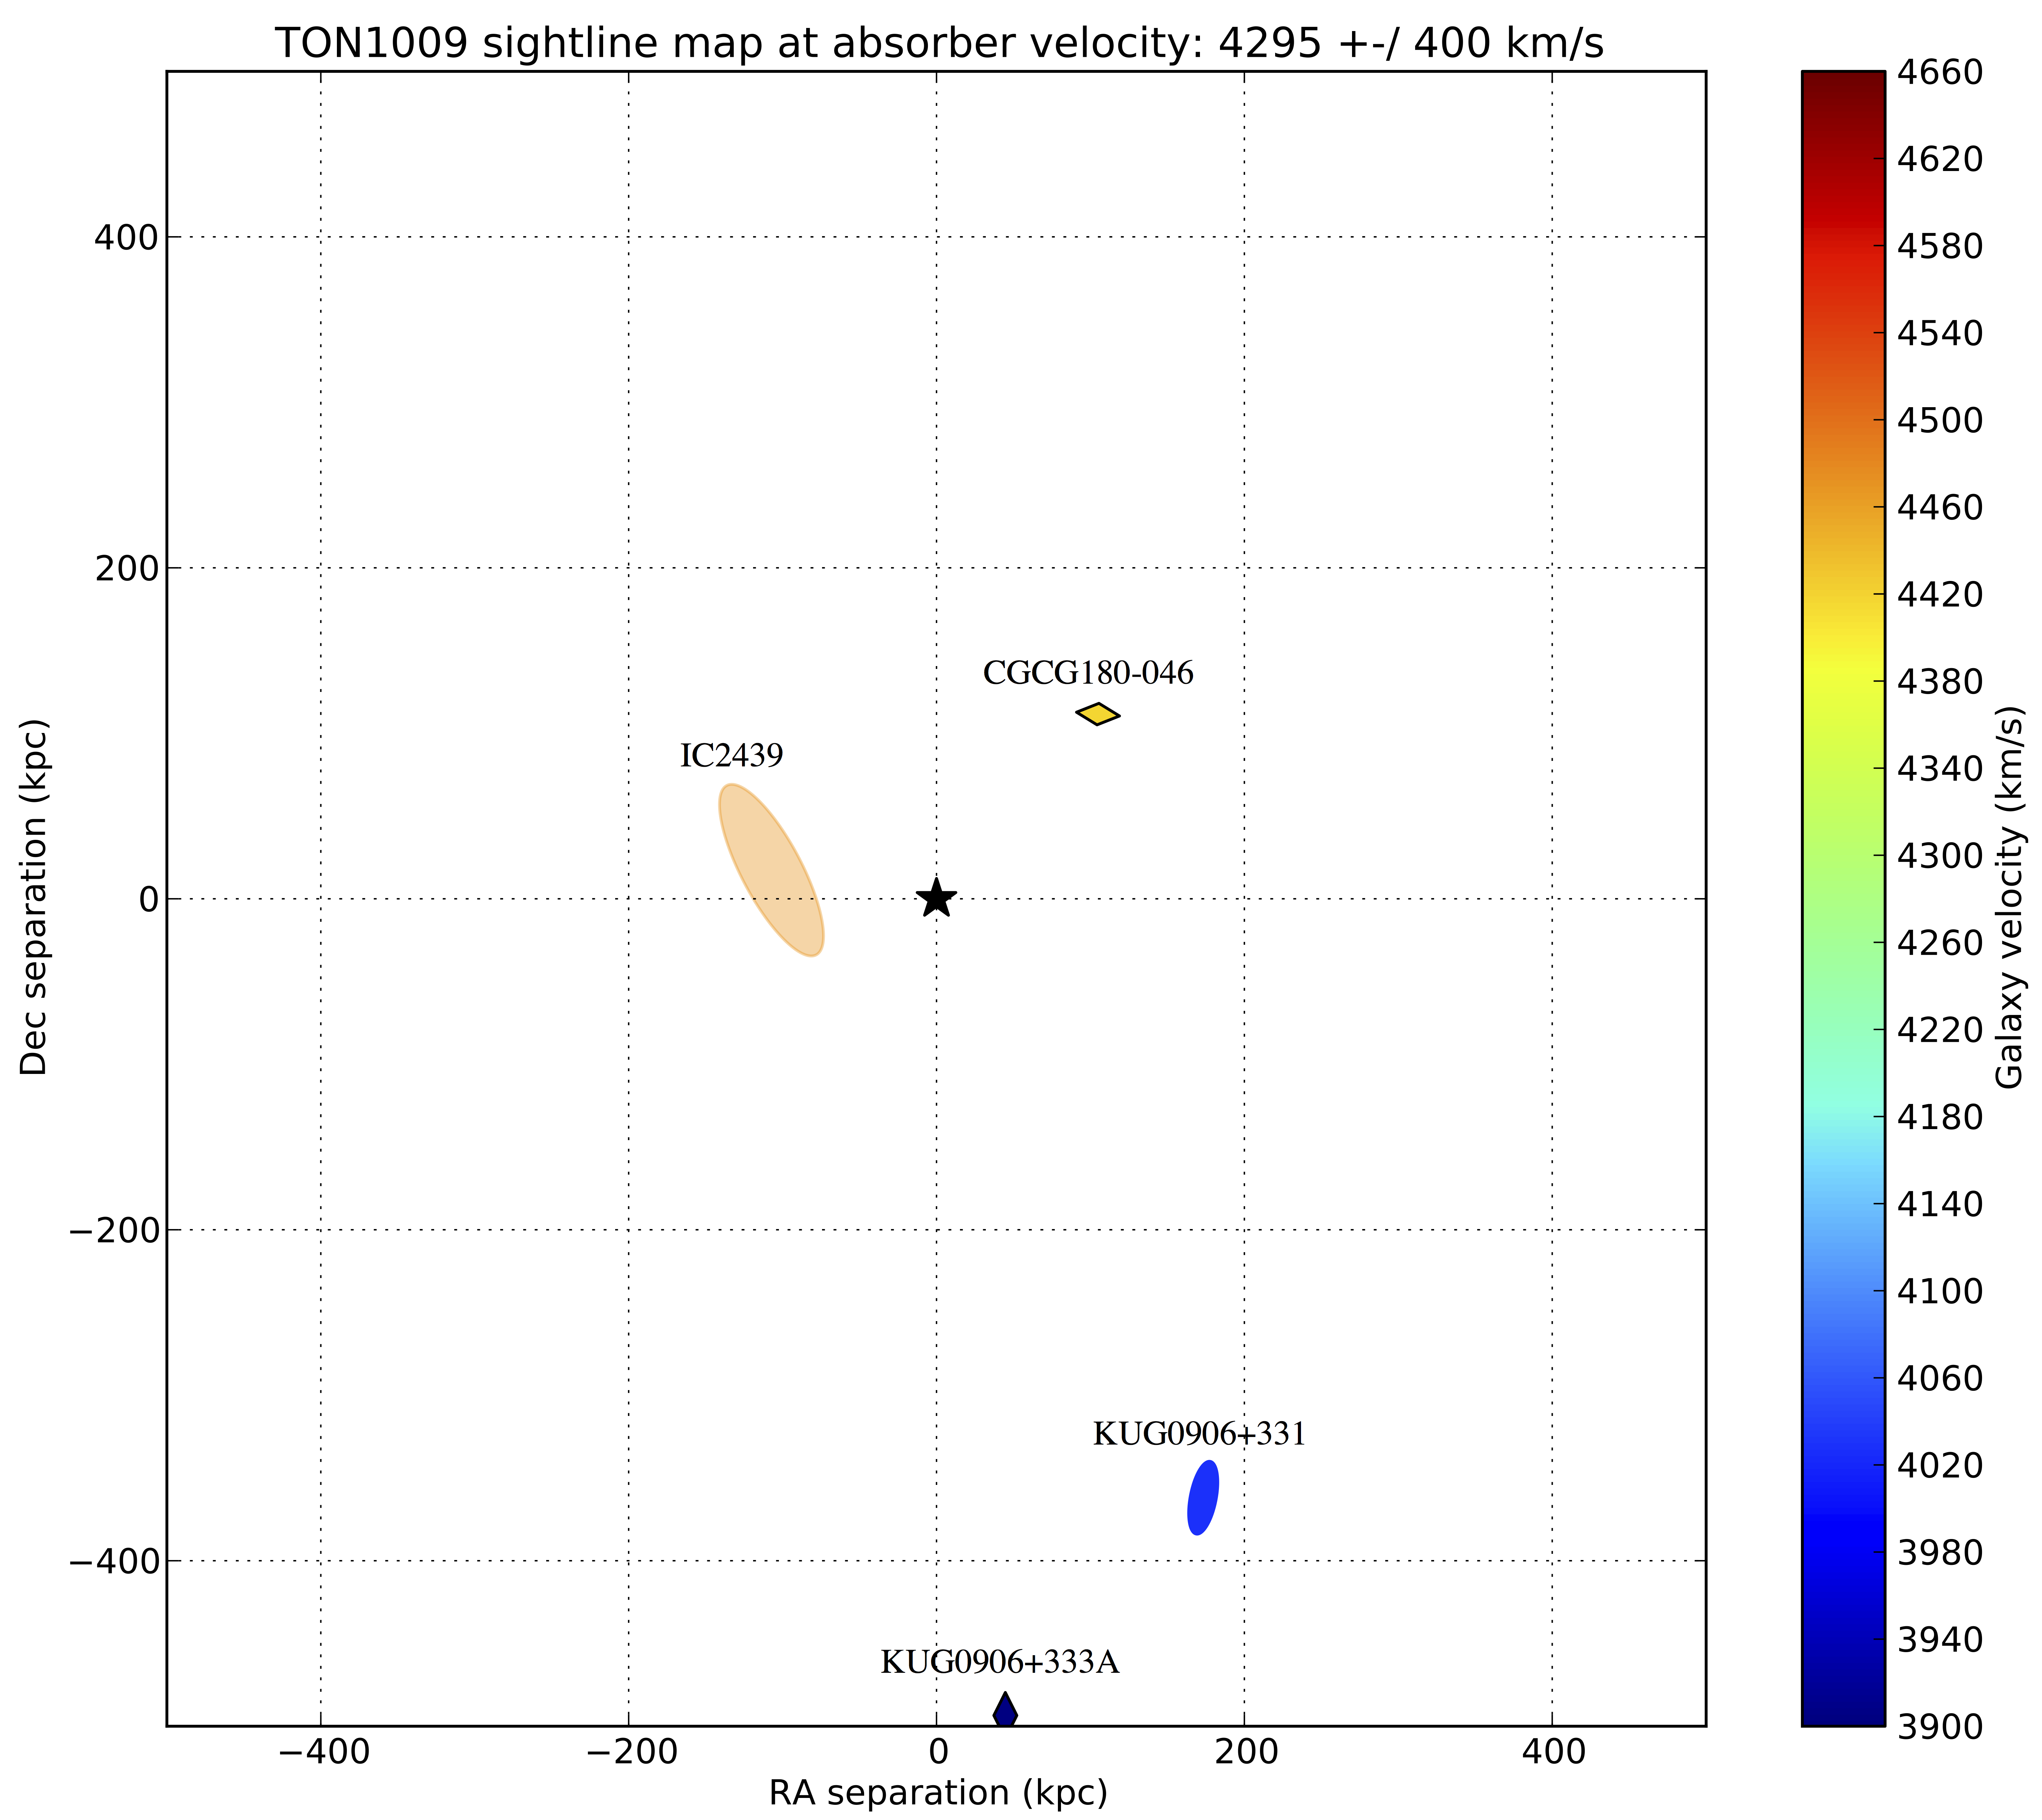
\includegraphics[width=1.\linewidth]{map2_TON1009_4295_newlabels_crop_hires2.png}\label{impactmap}}
  \caption{\small{a) An example Ly$\alpha$ line found in a sightline towards target TON1009 at 4295 km/s. b) A map of \textit{all} galaxies within a 500 kpc impact parameter target TON1009 sightline and with velocity ($cz$) within 400 km/s of absorption detected at 4295 km/s (central black star). The galaxy IC2439 ($v=4494$ km/s, inclination = $71^{\circ}$) can be unambiguously paired with the Ly$\alpha$ absorption feature at $v=4295$ km/s because it is the largest and closest galaxy in both physical and velocity space to the absorption feature.}}
\vspace{5pt}
\end{figure}


\section{Results}

We have identified 154 Ly$\alpha$ absorption lines in the spectra of 35 background QSOs. Of these, $32\%$ can be unambiguously associated with a single nearby galaxy, while $51\%$ reside in relative voids. In order to be considered for a pairing, a galaxy and absorption feature must appear within 400 km/s in velocity and 500 kpc in physical impact parameter from each other. When multiple galaxies pass these criteria for a particular line, we are left with two options. 1) one galaxy is obviously far larger and closer in physical and velocity space to the line, and may have several satellite galaxies, or 2) no single galaxy if obviously dominant, and we do not include this line in further analysis. 

To facilitate this decision, we compute the likelihood, $\mathcal{L}$, of every possible galaxy-absorber pairing as follows:

\begin{equation}
	\mathcal{L} = A e^{-(\frac{\rho}{R_{vir}})^2} e^{-(\frac{\Delta v}{200})^2}.
\end{equation}

\noindent Here $\rho$ is the physical impact parameter, $R_{vir}$ the virial radius of the galaxy, $\Delta v$ the velocity difference between the absorber and the galaxy ($\Delta v = v_{galaxy} - v_{absorber}$), and $A$ is a factor included to increase the likelihood in the case that $R_{vir} \geq \rho$ (in which case $A = 2$, otherwise $A = 1$). An absorber-galaxy system separated by 200 km/s in velocity and 1$R_{vir}$ would have $\mathcal{L} = 0.27$. In order for an absorber to be marked as ``associated" with a particular galaxy, its $\mathcal{L}$ must be a factor of 5 larger than the next best possible association. 

Figures \ref{line} and \ref{impactmap} show a clean example of a Ly$\alpha$ absorption line with a map of its galaxy environment, showing an unambiguous pairing between the absorption feature at $4295km/s$ toward TON1009 and galaxy IC2439 ($\mathcal{L} = 0.45$). Unless explicitly stated, all following analysis concerns similarly unambiguous ``associated" systems.



%\begin{figure}[h!]
%\centering
%  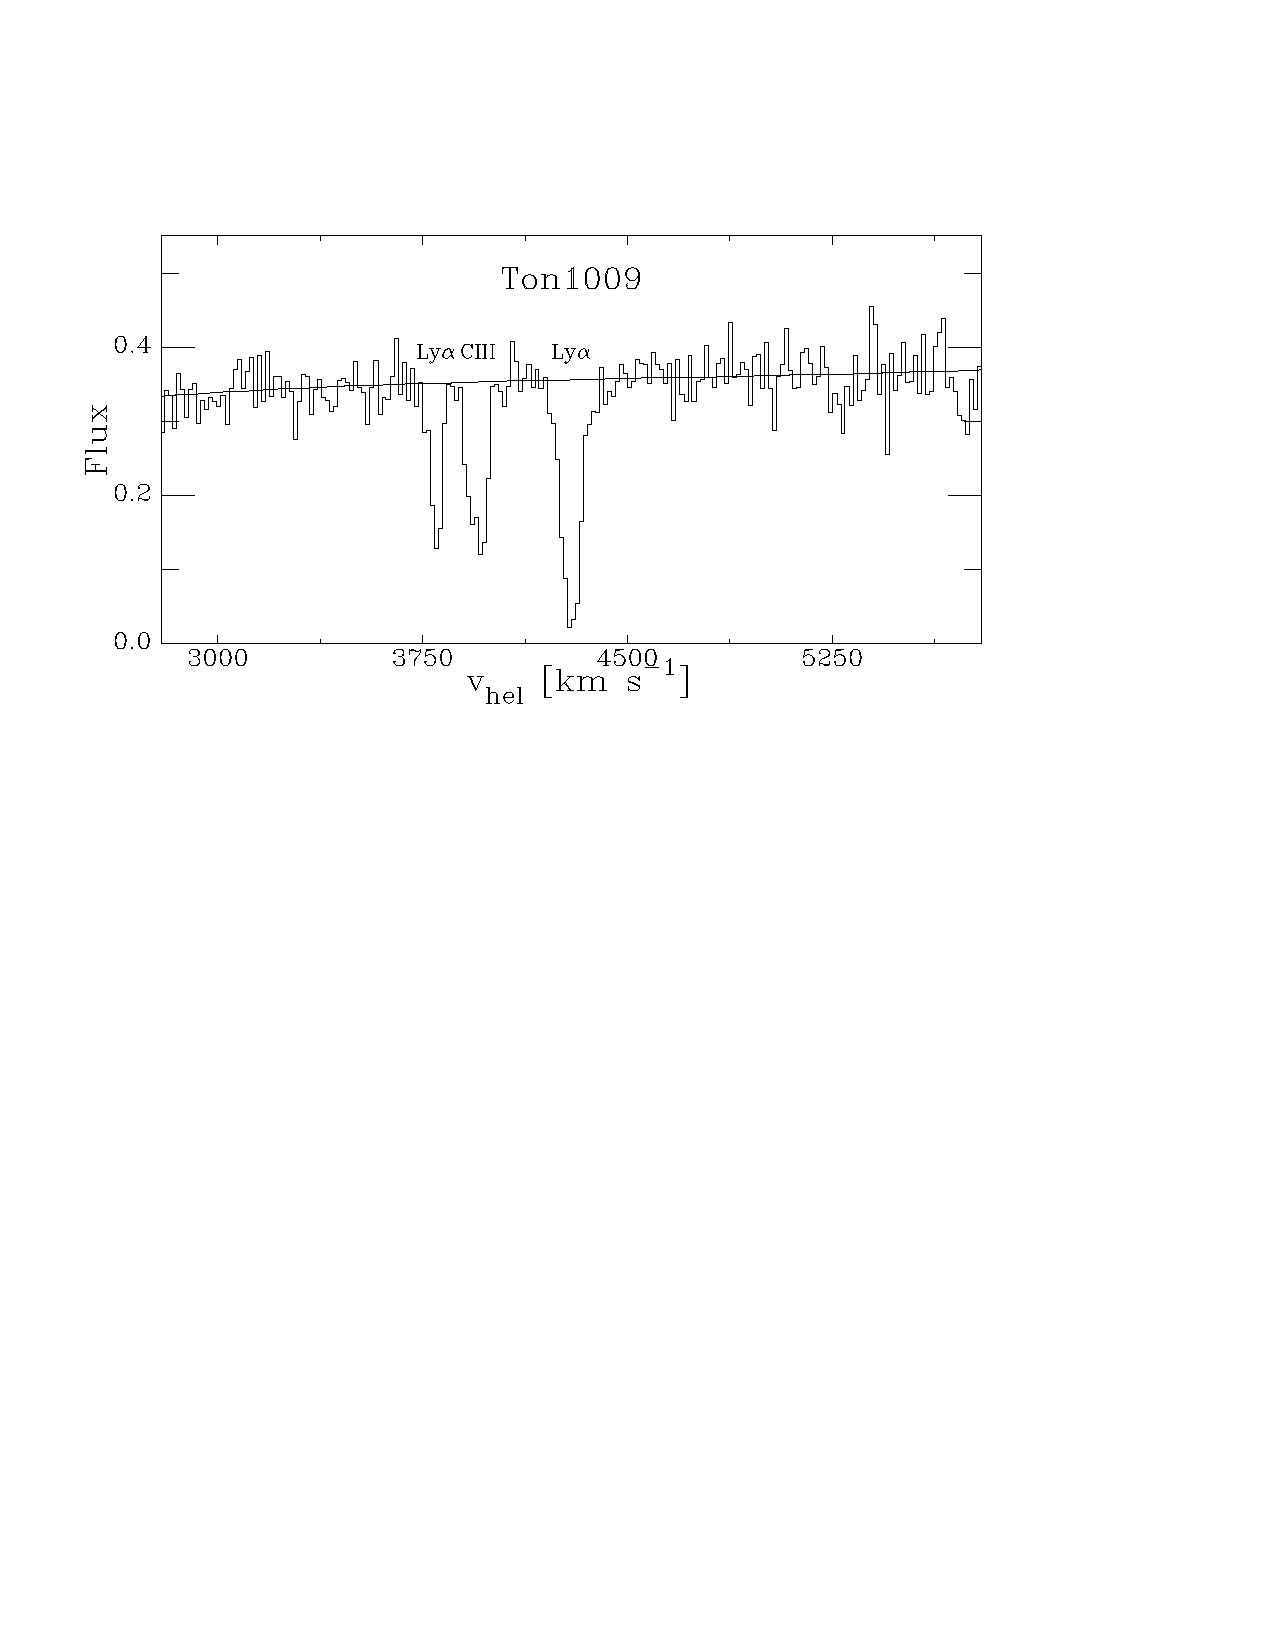
\includegraphics[width=1.\linewidth]{figTON1009_crop.pdf}
%  \caption{\small{An example Ly$\alpha$ line found in a sightline towards target TON1009 at 4295 km/s.}}
%  \label{line}
%\end{figure}
%\begin{figure}[h!]
%  \centering
%  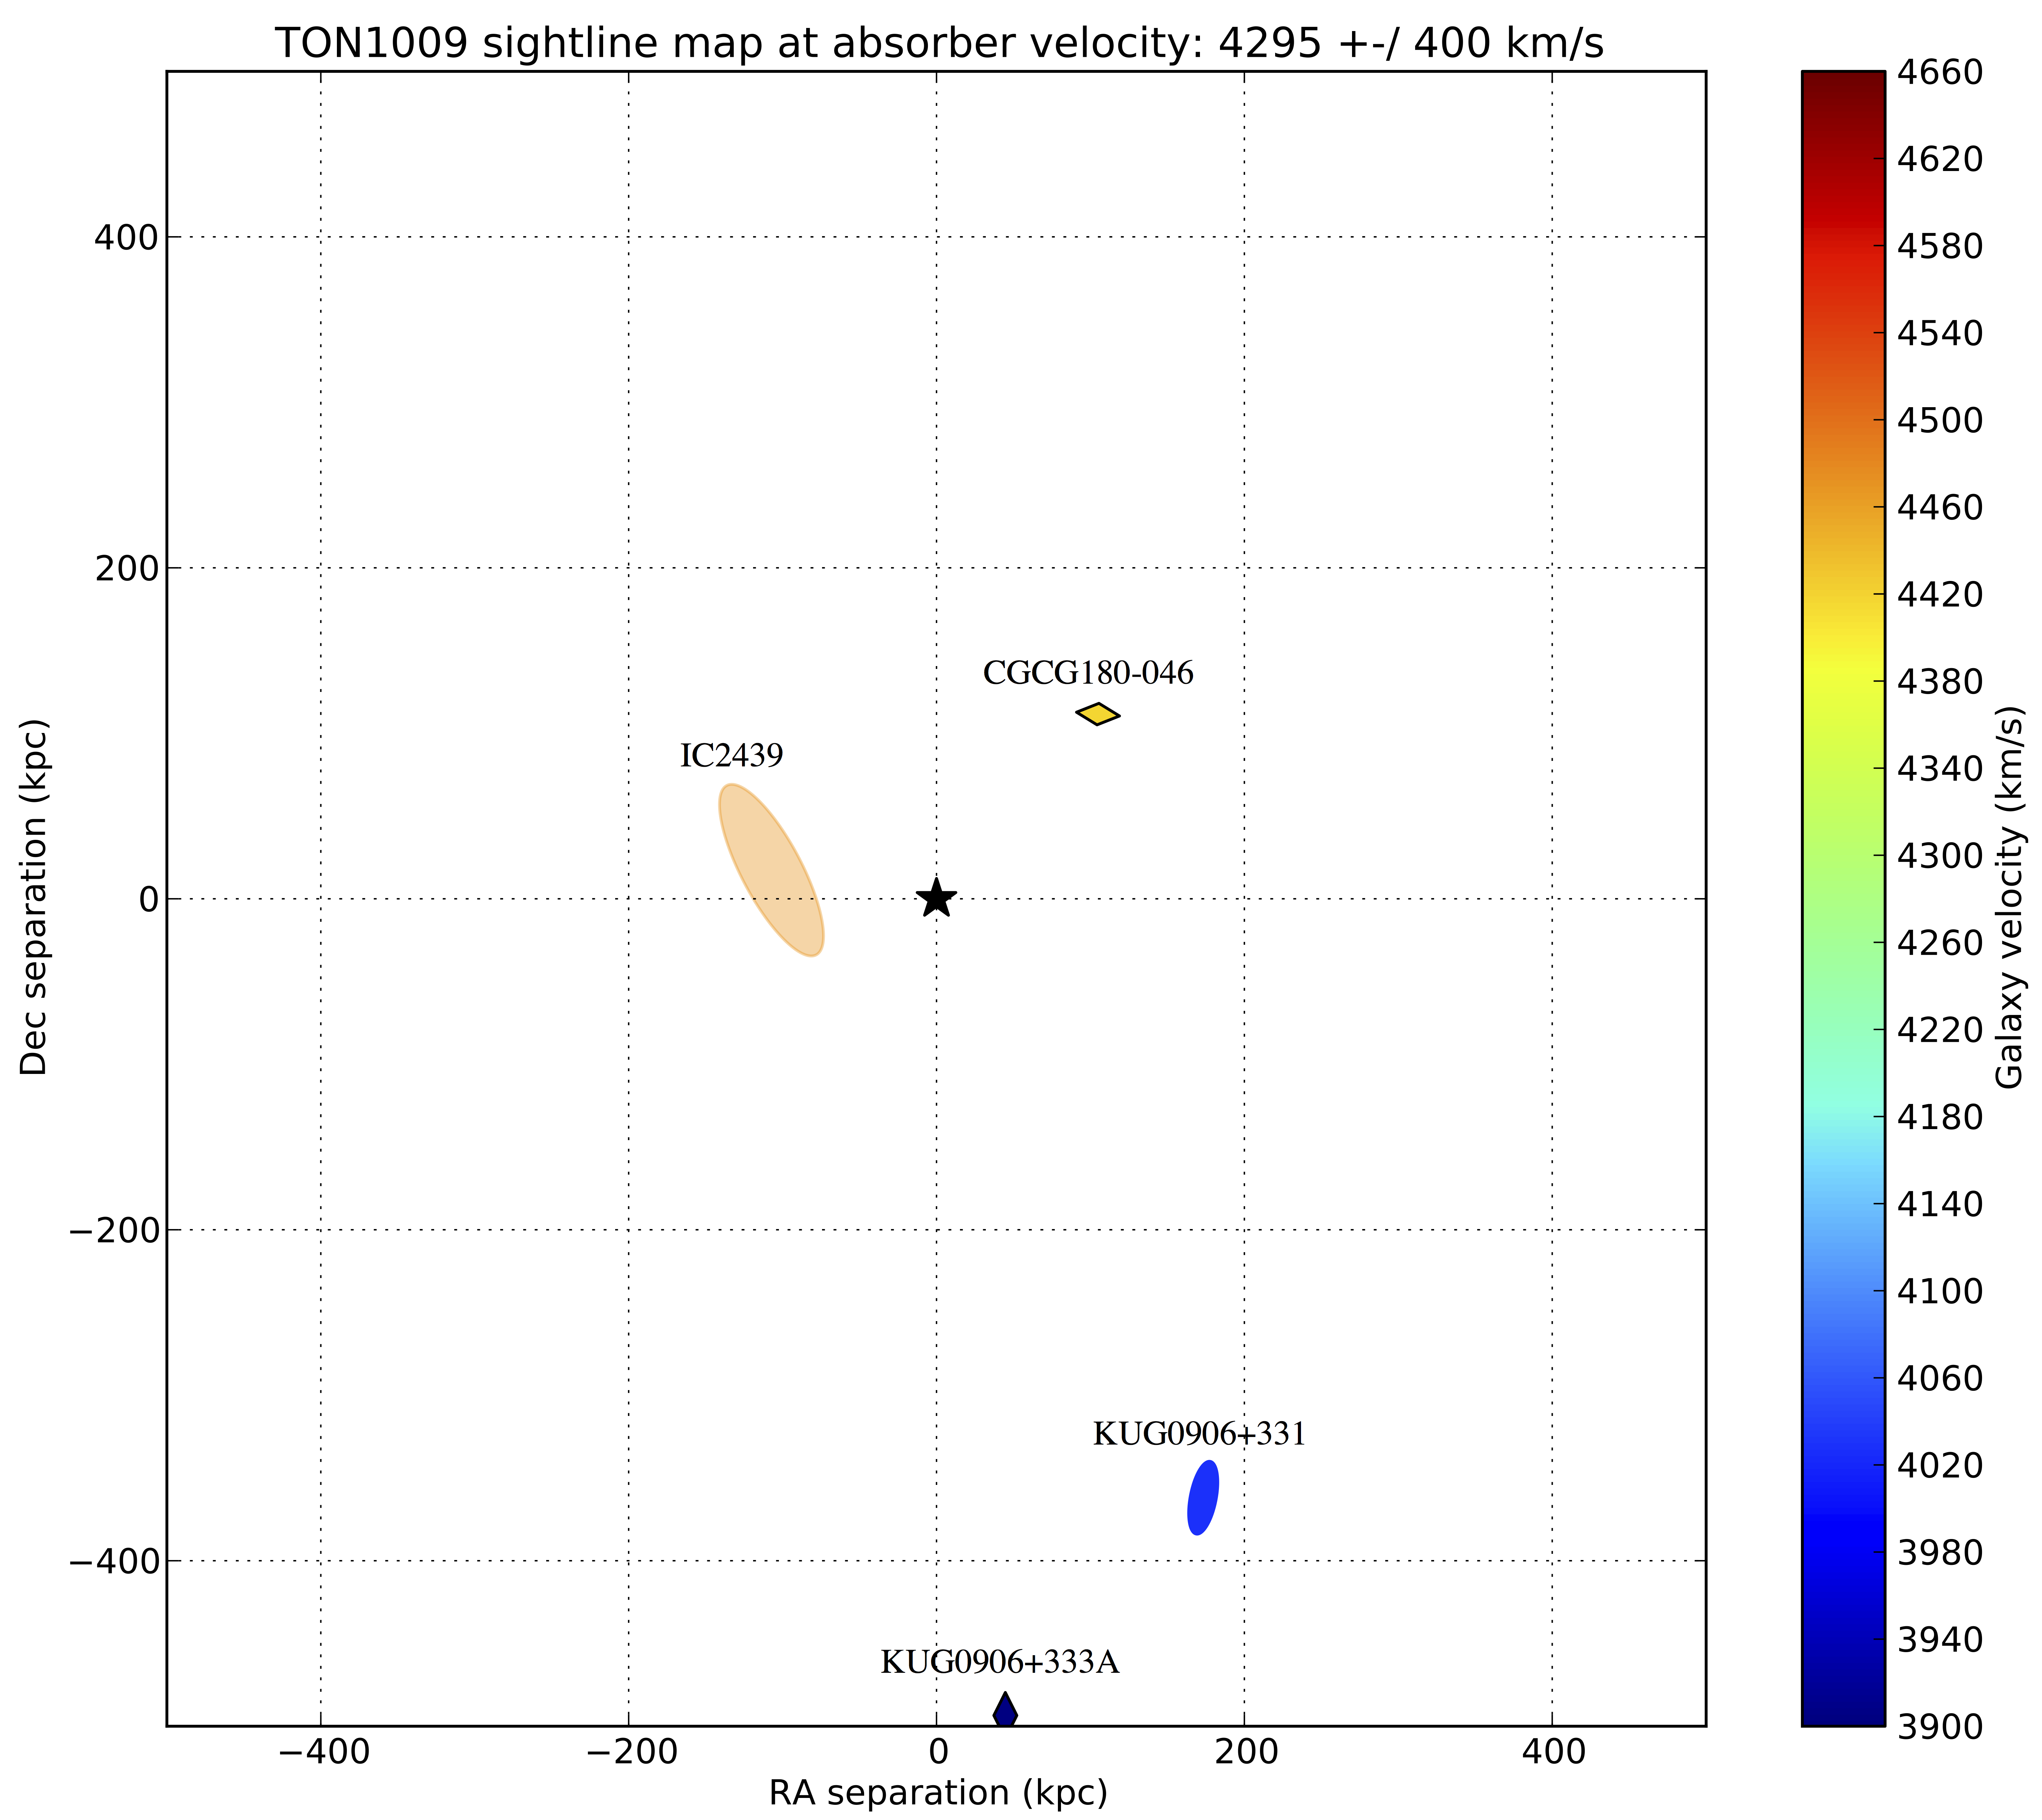
\includegraphics[width=1.\linewidth]{map2_TON1009_4295_newlabels_crop_hires2.png}
%  \caption{\small{A map of \textit{all} galaxies within a 500 kpc impact parameter target TON1009 sightline and with velocity ($cz$) within 400 km/s of absorption detected at 4295 km/s (central black star). The galaxy IC2439 ($v=4494$ km/s, inclination = $71^{\circ}$) can be unambiguously paired with the Ly$\alpha$ absorption feature at $v=4295$ km/s because it is the largest and closest galaxy in both physical and velocity space to the absorption feature.}}
%  \label{impactmap}
%\label{TON1009}
%\vspace{5pt}
%\end{figure}


\subsection{W-$\rho$ Anti-correlation}
As mentioned earlier, numerous previous studies have found that Ly$\alpha$ equivalent width (EW) is anti-correlated with impact parameter ($\rho$) to the nearest galaxy. We find this to be true only when normalizing impact parameters by the galaxy diameter. Figure \ref{ew_vs_impact} shows a straight comparison between Ly$\alpha$ $EW$ and $\rho$, where no correlation either way is apparent. Figure \ref{ew_vs_impact-d} shows that the expected anti-correlation clearly emerges when plotting $EW$ vs $\rho/diameter$. The obvious explanation for this is that larger galaxies host larger, more physically extent CGM halos. \textbf{NEED TO PLOT $\rho/R_{VIR}$ INSTEAD}


%\begin{figure*}[h!]
%\centering
%\begin{minipage}[b]{.49\textwidth}
%        \includegraphics[width=0.52\textwidth]{W(impact)_dif.pdf}
%        \caption{\small{Equivalent width ($W$) of each absorber as a function of $\rho$ (kpc), the physical impact parameter between the galaxy and the sightline toward the absorption feature. Only a slight anti-correlation can be seen.}}
%        \label{ew_vs_impact}
%\end{minipage}\hfill
%\begin{minipage}[b]{.49\textwidth}
%        \includegraphics[width=0.52\textwidth]{W(impact_diam)_dif.pdf}
%        \caption{\small{Equivalent width ($W$) of each absorber as a function of $\rho$/D, the ratio of the physical impact parameter and the galaxy diameter. A strong anti-correlation is evident.}}
%%        \vspace{-5pt}
%        \label{ew_vs_impact-d}
%\end{minipage}
%\end{figure*}




%\begin{figure}[h!]
%        \centering
%        \vspace{-10pt}
%        \includegraphics[width=0.52\textwidth]{W(impact)_dif.pdf}
%        \caption{\small{Equivalent width ($W$) of each absorber as a function of $\rho$ (kpc), the physical impact parameter between the galaxy and the sightline toward the absorption feature. Only a slight anti-correlation can be seen.}}
%%        \vspace{-5pt}
%        \label{ew_vs_impact}
%\end{figure} 
%
%\begin{figure}[h!]
%        \centering
%        \vspace{-10pt}
%        \includegraphics[width=0.52\textwidth]{W(impact_diam)_dif.pdf}
%        \caption{\small{Equivalent width ($W$) of each absorber as a function of $\rho$/D, the ratio of the physical impact parameter and the galaxy diameter. A strong anti-correlation is evident.}}
%%        \vspace{-5pt}
%        \label{ew_vs_impact-d}
%\end{figure} 

Most interestingly, new results emerge when we split the absorber-galaxy catalog based on the velocity difference of the two. We define the differential velocity between the absorption and an associated galaxy as follows:

\begin{equation}
	\Delta v = v_{galaxy} - v_{absorber}.
\end{equation}

With this scheme, we refer to an absorber with a velocity \textit{lower} than the associated galaxy as \textit{blueshifted}, while an absorber with a velocity \textit{higher} is referred to as \textit{redshifted}. The rest of the results will be analyzed based upon this splitting. For all distributions, we employ and quote the results of both the Kolmogorov-Smirnov (KS) and the Anderson-Darling (AD) statistical tests.

\begin{figure}[ht!]
  \centering
  \subfigure[]{\includegraphics[scale=0.44]{W(impact)_dif.pdf}}{\label{ew_vs_impact}}
  \subfigure[]{\includegraphics[scale=0.44]{W(impact_diam)_dif.pdf}}{\label{ew_vs_impact-d}}
  \vspace{-2pt}
  \caption{a) Equivalent width ($W$) of each absorber as a function of $\rho$ (kpc), the physical impact parameter between the galaxy and the sightline toward the absorption feature. b) ($W$) as a function of $\rho$/D, the ratio of the physical impact parameter and the galaxy diameter. A strong anti-correlation is evident only when scaling $\rho$ by the galaxy diameter.}
\end{figure}
\vspace{10pt}


\subsection{Inclination}
In this section we examine the inclinations of the associated galaxies compared to the red and blueshifted distributions of absorbers. Figure \ref{ew_vs_inclination} shows red and blueshifted absorbers' EW plotted against the inclinations of their associated galaxies. We note that there is a clear dichotomy between the distributions, where blue shifted absorbers appear around nearly all inclinations of galaxies, but redshifted absorbers only appear near highly-inclined galaxies (i.e. inclination $>$ 50 deg). In addition, redshifted absorbers appear with lower $W$ than those blueshifted across all inclinations. The average equivalent width of all redshifted absorbers is $\langle W \rangle$ = $192 \pm 12 \textrm{m\AA}$, compared to $\langle W \rangle$ = $366 \pm 15\textrm{m\AA}$ for blueshifted absorbers. We can reject the null hypothesis that red and blue shifted absorbers come from the same underlying distribution at the $95\%$ level (results of both KS and AD tests).


\subsection{Azimuth}
In this section we examine properties of absorbers as a function of their azimuthal angle with respect to their associated galaxy. Azimuth is defined as the angle between the major axis of a galaxy and the vector connecting the absorption feature and the midpoint of the galaxy plane. Figure \ref{azimuth} illustrates this. The mean azimuth angle for all absorption systems is \textbf{MEAN AZIMUTH ANGLE}. Again splitting the results into blue and redshifted bins leads to a slight separation in azimuth. We find a mean azimuth angle of \textbf{BLUESHIFTED AZIMUTH} for blue shifted absorbers, and \textbf{RED SHIFTED AZIMUTH} for redshifted absorbers. 


\begin{figure}[h!]
        \centering
        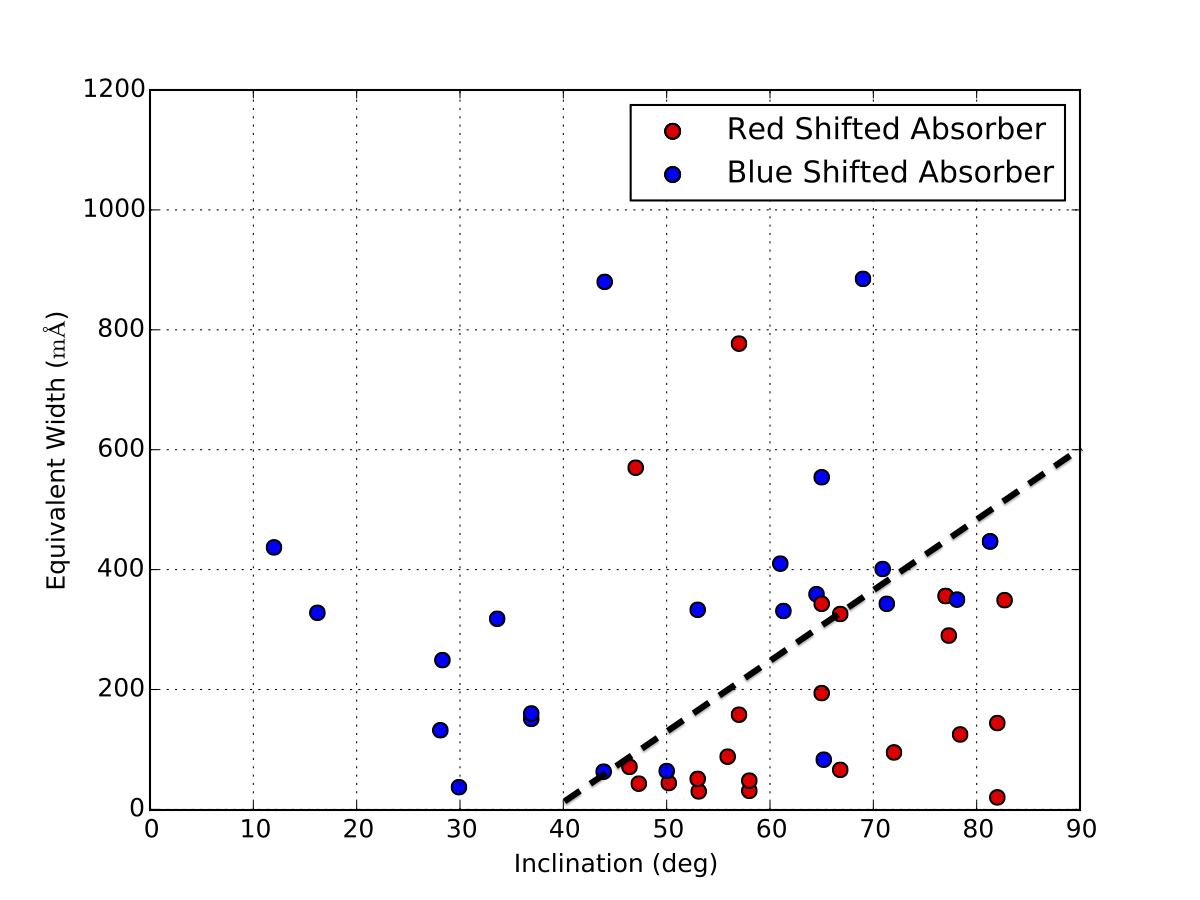
\includegraphics[width=0.52\textwidth]{Wvsinclinationfinal3.jpg}
        \caption{\small{Equivalent width ($W$) of each absorber as a function of the inclination angle of the associated galaxy in the pilot study sample. The dashed black line is drawn to highlight the separation between red and blue shifted absorption systems (with respect to the systemic velocity of the galaxy).}}
        \label{ew_vs_inclination}
\end{figure} 



%\begin{figure}[h!]
%        \centering
%        \vspace{-10pt}
%        \includegraphics[width=0.52\textwidth]{azimuth_explanation.jpg}
%        \caption{\small{Azimuth angle is defined to be the angle between the major axis of a galaxy, and a vector from the nucleus in the direction of the detected absorption. An azimuth angle of 0 deg describes an absorber lying along the plane of the major axis of the nearby galaxy.}}
%%        \vspace{-5pt}
%        \label{azimuth}
%\end{figure} 


We detect no significant difference between the diameter of the galaxies associated with red vs blue shifted absorbers.


\section{Discussion}


\textbf{WHAT'S THE MEAN $L_*$ OF ASSOCIATED GALAXIES? AND ALL THE FIELDS IN GENERAL?}


\nocite{*}
\bibliography{paper_bib}
\bibliographystyle{apj}

\end{document}
